\lecture{9}{2026.05.11}{}

\subsection{Convergence Rate}

Now we want to prove the convergence rate of Newton's method (Quadratic).

First, we assume $f$ satisfies that \begin{enumerate}
    \item $f$ is continuously differentiable
    \item $f'$ is Lipschitz continuous, i.e. \[
        \|f'(y) - f'(x)\| \leq \alpha \|y-x\|, \quad \forall x,y    
    \]
    where $\alpha > 0$ is the Lipschitz constant.
\end{enumerate}

\begin{theorem}
    If $\{x^k\} \to x^*$ and $f'(x^*) \neq 0$, then \begin{enumerate}
        \item $f(x^*) = 0$
        \item $\exists L \ge 1,\ \delta > 0$ such that $\forall k \ge L$ \[
            \|x^{k+1} - x^*\| \leq \delta \|x^k - x^*\|^2        
        \]
    \end{enumerate}
    \begin{note}
        For this theorem, we call it ``local convergence analysis'' since we need the sequence $\{x^k\}$ to converge to $x^*$ first.
    \end{note}
\end{theorem}
\begin{proof}[Proof 1]
    For the first part, from the update rule of Newton's method and Lemma \ref{lemma:con}, \begin{align*}
        f(x^{k+1}) &= f(x^k) + f'(x^k)(x^{k+1} - x^k) + e(x^{k+1}, x^k) \\
        &= e(x^{k+1}, x^k)
    \end{align*}
    where \[
        |e(x^{k+1}, x^k)| \leq \frac{\alpha}{2} \|x^{k+1} - x^k\|^2
    \]
    Thus, \[
        |f(x^{k+1})| \leq \frac{\alpha}{2} \|x^{k+1} - x^k\|^2
    \]
    Since $\{x^k\} \to x^*$, and the above inequality holds, we have \[
        |f(x^{k+1})| \to 0
    \]
    Since $f$ is continuous, we have \[
        f(x^{k+1}) \to f(x^*) \mbox{ implies } f(x^*) = 0
    \]
\end{proof}
\begin{proof}[Proof 2]
    For the second part, we define \[
        \bar{\beta} \equiv |f'(x^*)^{-1}|
    \]
    Since \[
        |x^{k} - x^*| \to 0
    \]
    and $f'$ is Lipschitz continuous, $\exists L \ge 1$ such that $\forall k \ge L$ 
    \begin{eqnarray*}
    |f'(x^*)^{-1} (f'(x^k)-f'(x^*))|
    & \leq &   
    |f'(x^*)^{-1}| |f'(x^k)-f'(x^*)| \\
    & \leq & \alpha \bar{\beta} |x^k - x^*|\\
    & \leq & \frac{1}{2}
    \end{eqnarray*}
    For $k \ge L$, from Lemma \ref{lemma:bound}, $f'(x^k)^{-1}$ exists and \begin{equation}
        |f'(x^k)^{-1}| \leq 2 \bar{\beta} \label{eq:bound_res}
    \end{equation}
    By definition of Newton's method, \begin{equation}
        x^{k+1} - x^* = x^k - x^* - f'(x^k)^{-1} f(x^k) \label{eq:updatebound}
    \end{equation}
    Since $f(x^*) = 0$, we have \[
        f(x^*) = f(x^k) + f'(x^k)(x^* - x^k) + e(x^*, x^k) = 0
    \]
    Then multiply both sides by $f'(x^k)^{-1}$, we have \begin{equation}
        f'(x^k)^{-1} f(x^k) = x^k - x^* - f'(x^k)^{-1} e(x^*, x^k) \label{eq:res_bound} 
    \end{equation}
    Thus, (\ref{eq:bound_res}) and (\ref{eq:updatebound}) imply \begin{equation}
        x^{k+1} - x^* = f'(x^k)^{-1} e(x^*, x^k) \label{eq:final_bound}
    \end{equation}
    From (\ref{eq:bound_res}) and (\ref{eq:res_bound}), and Lemma \ref{lemma:con}, for $k \ge L$, 
    \begin{eqnarray*}
        |x^{k+1} - x^*| & \leq & 
        |f'(x^k)^{-1}|
        |e(x^*,x^k)|\\
        & \leq & 2\bar{\beta}\frac{1}{2}
        \alpha 
        |x^{k} - x^*|^2  \\
        & = & \delta
        |x^{k} - x^*|^2,  
    \end{eqnarray*}
    where we define \[
        \delta = \alpha \bar{\beta}
    \]
    Then proof is complete.
\end{proof}

\begin{lemma} \label{lemma:bound}
    If \begin{equation}
        |f'(x^*)^{-1} (f'(x^k)-f'(x^*))| \leq 1 \label{eq:bound1}
    \end{equation}
    then \begin{equation}
        |f'(x^k)^{-1}| \leq \frac{|f'(x^*)^{-1}|}{1 - |f'(x^*)^{-1} (f'(x^k)-f'(x^*))|} \label{eq:bound2}
    \end{equation}
\end{lemma}
\begin{proof}
    The inequality (\ref{eq:bound2}) \begin{equation*}
        |f'(x^k)^{-1}| \leq \frac{|f'(x^*)^{-1}|}{1 - |f'(x^*)^{-1} (f'(x^k)-f'(x^*))|}
    \end{equation*}
    is equivalent to \begin{eqnarray}
    && |f'(x_k)^{-1}|
    - |f'(x^*)^{-1} - f'(x_k)^{-1}| \nonumber
    \\
    &= & |f'(x_k)^{-1}|
    - | f'(x_k)^{-1} - f'(x^*)^{-1}| \nonumber
    \\  
    & \leq & |f'(x^*)^{-1}|, \label{eq:3}
    \end{eqnarray}
    where the last inequality is from the property of absolute values.
    \begin{note}
        We need the condition (\ref{eq:bound1}) to ensure that the denominator in (\ref{eq:bound2}) is positive, which is necessary for the inequality to hold.
    \end{note}
    Proof complete.
\end{proof}

\begin{lemma} \label{lemma:con}
    If $f'$ is Lipschitz continuous with constant $\alpha>0$, and \[
        f(y) = f(x) + f'(x)(y-x) + e(y,x)
    \]
    then \[
        |e(y,x)| \leq \frac{\alpha}{2} |y-x|^2    
    \]
\end{lemma}
\begin{proof}
    Because \[
        \frac{d}{dt} f(x+t(y-x)) = f'(x + t(y-x))(y-x)
    \]
    we have \begin{eqnarray*}
        && \int_0^1 (f'(x+t(y-x))-f'(x))(y-x)dt  \\
        & = & \left(\int_0^1 f'(x+t(y-x))(y-x)dt\right) - f'(x)(y-x)\\
        & = & f(x+t(y-x))\Bigr\rvert^{1}_{t=0} 
                - f'(x)(y-x)\\  
        & = & f(y) - f(x) - f'(x)(y-x)
    \end{eqnarray*}
    then \begin{eqnarray}
    |e(y,x)|
    & \leq & 
    \int_0^1 |(f'(x+t(y-x))-f'(x))(y-x)|dt    \label{eq11} \\
    & \leq & 
    \int_0^1 \alpha |(x+t(y-x))-x||(y-x)| dt    \label{eq21} \\
    & \leq & 
    \int_0^1 \alpha t |(y-x)|^2 dt \ = \ \boxed{\frac{1}{2} \alpha |y-x|^2}, \nonumber
\end{eqnarray}
    where (\ref{eq11}) to (\ref{eq21}) is from the Lipschitz condition of $f'$.
\end{proof}

\chapter{Interpolation and Approximation}

If $f^{(n)}(x)$, $\forall n$ are available, Taylor's polynomial is an approximation: \[
    f(x) = f(x_0) + f'(x_0)(x-x_0) + \frac{1}{2!} f''(x_0)(x-x_0)^2 + \cdots 
\]
\begin{eg}
    \[
        e^x  = 1 + \frac{x}{1!} + \frac{x^2}{2!} + \frac{x^3}{3!} + \cdots
    \]
\end{eg}

In this approximation, we only need information of \red{one point}. If finite terms are used, the approximation can only be accurate near $x_0$. Primal use of Taylor's polynomial for numerical methods is the derivation of numerical techniques but not for approximation. Subsequently, we discuss some techniques of \textbf{interpolation} and \textbf{approximation}

\begin{definition}[Interpolation]
    Find a function passing all the given data points, i.e. \[
        f(x_i) = y_i, \quad i = 1,2,\cdots,n
    \]
\end{definition}

\begin{definition}[Approximation]
    Find a function that error to the given data points is small, i.e. \[
        |f(x_i) - y_i| \leq \epsilon, \quad i = 1,2,\cdots,n
    \]
\end{definition}

\section{Interpolation}

\subsection{Lagrange Polynomial}

Given $(x_0, f(x_0)), (x_1, f(x_1)), \cdots, (x_n, f(x_n))$, find a polynomial $P_n(x)$ of degree at most $n$ passing through these points.

\begin{note}
    This is the simplest form of functions.
\end{note}

Degree $1$ polynomial passing two points is a straight line.

\begin{eg}
    Given $(x_0, f(x_0)), (x_1, f(x_1))$.
\end{eg}

Define \[
    L_0(x) \equiv \frac{x-x_1}{x_0 - x_1}, \quad L_1(x) \equiv \frac{x-x_0}{x_1 - x_0}
\]
\[
    P_1(x) = L_0(x) f(x_0) + L_1(x) f(x_1)
\]
Then \[
    P_1(x_0) = f(x_0), \quad P_1(x_1) = f(x_1)
\]

\begin{eg}
    For the general case with $n+1$ points. Consider a polynomial with degree at most $n$ \[
        (x_0, f(x_0)), (x_1, f(x_1)), \cdots, (x_n, f(x_n))
    \]
\end{eg}

\begin{definition}[Lagrange polynomial]
    Construct $L_{n,k}(x)$ as \[
        L_{n,k}(x_i) = \begin{cases}
            1, & i = k \\
            0, & i \neq k
        \end{cases}
    \]
    where $n$ is the degree of the polynomial, and $k$ is the index of the point. Then \[
        P_n(x) = \sum_{k=0}^n L_{n,k}(x) f(x_k)
    \]
\end{definition}

Thus we have \[
    P_n(x_i) = f(x_i), \quad i = 0,1,\cdots,n
\]

\begin{definition}[Lagrange basis polynomial]
    The Lagrange basis polynomial $L_{n,k}(x)$ is defined as \[
        L_{n,k}(x) \equiv \prod_{j=0, j \neq k}^n \frac{x-x_j}{x_k - x_j}
    \]
\end{definition}

\subsection{Spline Interpolation}

Using Lagrange polynomial is bad since \begin{enumerate}
    \item The degree of the polynomial is high.
    \item There is a large fluctuation between the data points, which is called Runge's phenomenon.
\end{enumerate}

A piecewise polynomial is a better choice.

\begin{definition}[Linear spline]
    A series of straight lines connecting the data points \[
        (x_0, f(x_0)), (x_1, f(x_1)), \cdots, (x_n, f(x_n))
    \]
\end{definition}

\begin{eg}
\begin{equation*}
    x= 
    \begin{bmatrix}
    0 & 1 & 2 & 3
    \end{bmatrix},
    y = 
    \begin{bmatrix}
    0 & 1 & 4 & 3  
    \end{bmatrix}
\end{equation*}
\end{eg}

\begin{figure}[H]
    \centering
    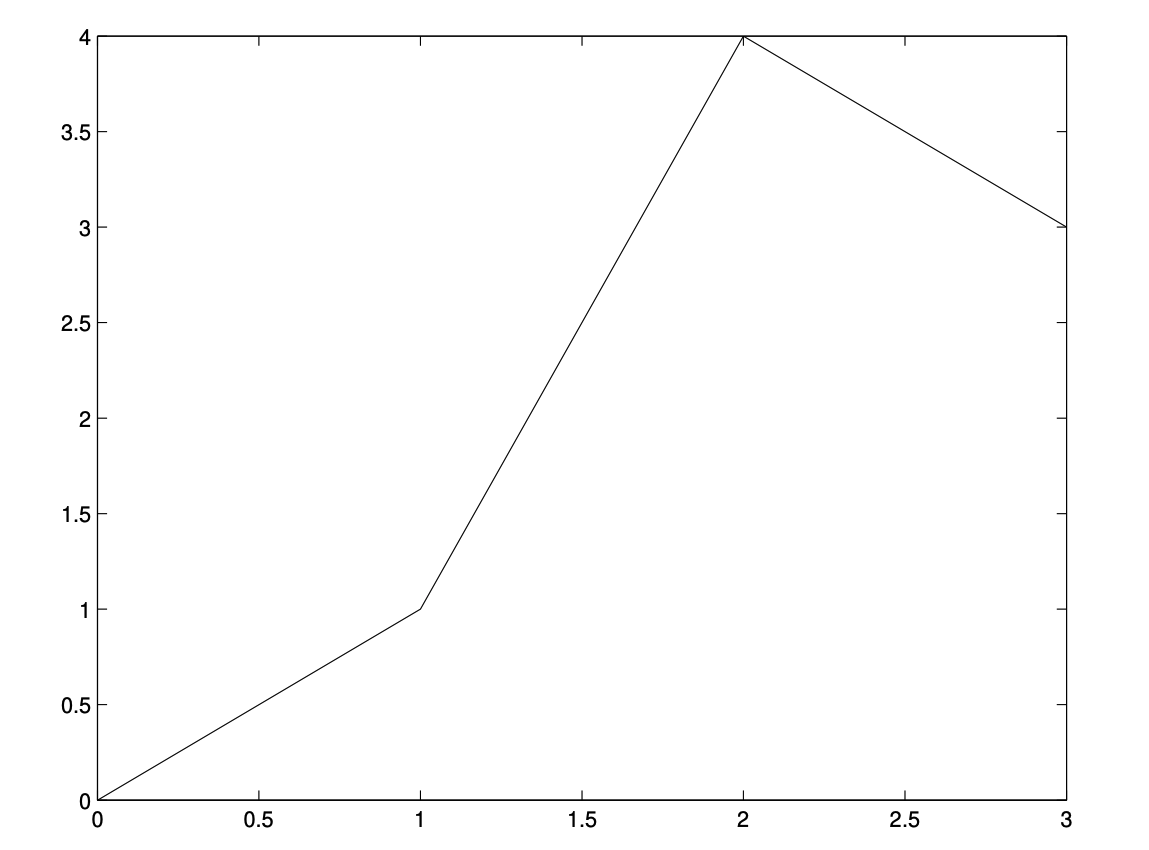
\includegraphics[width=0.27\textwidth]{Figures/linearspline.png}
    \caption{Linear spline interpolation}
\end{figure}

\begin{definition}[Linear spline interpolation]
    Define $s_0(x), s_1(x), \cdots, s_{n-1}(x)$ as \[
        s_j(x) = \frac{x_{j+1} - x}{x_{j+1} - x_j} f(x_j) + \frac{x - x_j}{x_{j+1} - x_j} f(x_{j+1}), \quad x_j \leq x \leq x_{j+1}
    \]
\end{definition}

However, linear spline is not smooth, which is not differentiable at the data points. Thus, we need a smoother interpolation. A possiblilty is to use higher degree $s_j(x)$ and hope that \[
    s'_0(x), s'_1(x), \cdots, s'_{n-1}(x)
\]
are continuous.

Thus, the requirement is \begin{gather*}
    s_j(x_j) = f(x_j), j = 0,\ldots, n-1, \\
    s_{n-1}(x_n) = 
    f(x_n) \nonumber
    \\
    s_{j+1}(x_{j+1}) = s_j(x_{j+1}), j = 0, \ldots, n-2
    \\
    s_{j+1}'(x_{j+1}) = s_j'(x_{j+1}), j=0, \ldots, n-2    
\end{gather*}


\begin{note}
    We have \[
        n + 1 + 2(n-1) = 3n - 1
    \]
    conditions. A quadratic piecewise interpolation has $3n$ parameters, which is more than the number of conditions. For each interval, we can set $3$ parameters.
\end{note}

Nowadays, cubic spline interpolation is the most popular choice, which has another name ``\textbf{Spline}'' which use $4n$ parameters.


\begin{gather}
s_j(x_j) = f(x_j), j = 0,\ldots, n-1, \label{a}\\
s_{n-1}(x_n) = 
f(x_n) \nonumber
\\
s_{j+1}(x_{j+1}) = s_j(x_{j+1}), j = 0, \ldots, n-2
\label{b} \\
s'_{j+1}(x_{j+1}) = s'_j(x_{j+1}), j = 0, \ldots, n-2 \nonumber\\
s''_{j+1}(x_{j+1}) = s''_j(x_{j+1}), j = 0, \ldots, n-2 \nonumber
\end{gather}

The number of conditions is \[
    n + 1 + 2(n-1) + (n-2) = 4n - 2
\]

From the view point of solving the system of equations, we have $4n$ parameters and $4n-2$ conditions, which means we need to set $2$ more conditions to make the system solvable.

The boundary conditions are \begin{gather*}
    s''_0(x_0) = 0, s''_{n-1}(x_n) = 0 \quad \mbox{(natural spline)} \\
    s'_0(x_0) = f'(x_0), s'_{n-1}(x_n) = f'(x_n) \quad \mbox{(clamped spline)}
\end{gather*}

Now we have $4n$ conditions, hence the system is solvable. 

\begin{definition}[Cubic spline interpolation]
    Construct cubic polynomials
    \[
        s_j(x) \equiv a_j + b_j (x-x_j) + c_j (x-x_j)^2 + d_j (x-x_j)^3, \quad j = 0,1,\cdots,n-1
    \]
\end{definition}


Immediately, \[
    s_j(x_j) = a_j = f(x_j), \quad j = 0,1,\cdots,n-1
\]

Now (\ref{b}) becomes \[
    a_{j+1} = a_j + b_j(x_{j+1} - x_j) + c_j (x_{j+1} - x_j)^2 + d_j (x_{j+1} - x_j)^3, \quad j = 0,1,\cdots,n-2
\]

Now we define \begin{gather*}
h_j \equiv x_{j+1} - x_j \\
a_n \equiv f(x_n)
\end{gather*}
Earlier $a_j$ is only from $0$ to $n-1$.

We have \begin{equation*}
    a_n = s_{n-1}(x_n) = a_{n-1} + b_{n-1} h_{n-1} + c_{n-1} h_{n-1}^2 + d_{n-1} h_{n-1}^3
\end{equation*}

Then \begin{equation}
    a_{j+1} = a_j + b_j h_j + c_j h_j^2 + d_j h_j^3, \quad j = 0,1,\cdots,n-1 \label{eq:an}
\end{equation}

Now we define \begin{equation}
    b_n \equiv s'_{n-1}(x_n) \label{eq:bn}
\end{equation}
Earlier $b_j$ is only from $0$ to $n-1$.

Using 
\begin{gather}
    s'_j(x) = b_j+ 2c_j(x-x_j) + 3d_j(x-x_j)^2
    \nonumber \\
    s'_{j+1}(x_{j+1}) = s'_j(x_{j+1}),\; \; j = 0, \ldots, n-2  
    \nonumber \\
    b_{j+1} = b_j+ 2c_j h_j + 3d_j h_j^2, \; \;
    j = 0, \ldots, n-1
    \label{bj+1}
\end{gather}

Then we define \[
    c_n \equiv s''_{n-1}(x_n) /2
\]
Since \begin{gather*}
s''_{j+1}(x_{j+1}) = s''_j(x_{j+1}), 
\; \; j = 0, \ldots, n-2\\
s''_j(x) = 2c_j + 6d_j(x-x_j)\\
s''_j(x_{j+1}) = 2c_j + 6d_jh_j\\
s''_{j+1}(x_{j+1}) = 2c_{j+1}
\end{gather*}
we have \[
    c_{j+1} = c_j + 3d_j h_j, \quad j = 0, \ldots, n-1
\]
Thus \[
    d_j = \frac{c_{j+1} - c_j}{3h_j}
\]

\begin{note}
    This process is like Gaussian elimination, where we eliminate $a_j$ and $b_j$ to get a system of equations with only $c_j$.
\end{note}

Hence, (\ref{eq:an}) becomes \begin{eqnarray}
a_{j+1} 
&= &a_j + b_j h_j
+ c_j h_j^2
+ \frac{c_{j+1}-c_j}{3h_j} h_j^3\nonumber \\
&= &a_j + b_j h_j
+ \frac{h_j^2}{3}(2c_{j}+c_{j+1}),
\; \; j = 0, \ldots, n-1
\label{3.5}
\end{eqnarray}

And (\ref{bj+1}) becomes \begin{eqnarray}
b_{j+1} &= &b_j+ 2c_j h_j + 3d_j h_j^2 \nonumber\\
&=& b_j+ 2c_j h_j + 3\frac{c_{j+1}-c_j}{3h_j}
h_j^2 \nonumber\\
&=&  b_j+ 2c_j h_j + h_j(c_{j+1}-c_j)\nonumber\\
&=& b_j + h_j(c_j+c_{j+1}),
\; \; j = 0, \ldots,n-1
\label{3.6}
\end{eqnarray}

We have known $a_j$, unknown $b_j$ and $c_j$. 

From (\ref{3.5}) \[
    b_j = \frac{1}{h_j} (a_{j+1} - a_j) - \frac{h_j}{3}(2c_j + c_{j+1}), \quad j = 0,1,\cdots,n-1
\]
i.e. \[
    b_{j-1} = \frac{1}{h_{j-1}} (a_{j} - a_{j-1}) - \frac{h_{j-1}}{3}(2c_{j-1} + c_{j}), \quad j = 1,2,\cdots,n
\]
Rewriting (\ref{3.6}) \[
    b_j = b_{j-1} + h_{j-1}(c_{j-1}+c_j), \quad j = 1,2,\cdots,n
\]
and substituting the expression \begin{equation*}
\frac{1}{h_j}
(a_{j+1}-a_j) - \frac{h_j}{3}
(2c_{j}+c_{j+1}) =
\frac{1}{h_{j-1}}
(a_{j}-a_{j-1}) - \frac{h_{j-1}}{3}
(2c_{j-1}+c_{j}) + 
h_{j-1}(c_{j-1}+c_{j}),
j = 1, \ldots,n-1
\end{equation*}

\begin{note}
    \red{$j$ cannot be zero now.}
\end{note}

Finally, we have \begin{equation*}
\frac{h_{j-1}}{3} c_{j-1}  
+ \frac{2(h_{j-1} +h_j)}{3}c_j + 
\frac{h_j}{3} c_{j+1}
=\frac{1}{h_j}
(a_{j+1}-a_j)
-\frac{1}{h_{j-1}}
(a_{j}-a_{j-1})
\end{equation*}
so, \begin{eqnarray}
&& h_{j-1} c_{j-1}  
+ 2(h_{j-1} +h_j)c_j + h_j c_{j+1}\nonumber \\
&=&\frac{3}{h_j}
(a_{j+1}-a_j)
-\frac{3}{h_{j-1}}
(a_{j}-a_{j-1}), j=1, \ldots, n-1
\label{ajdiff}
\end{eqnarray}
The only unknowns are $c_j$, $j = 0,1,\cdots,n$. Once we solve $c_j$, we can solve $b_j$ and $d_j$. We see the boundary conditions. If $s''_0(x_0) = s''_{n-1}(x_n) = 0$, then \[
    s''_0(x) = 2c_0 + 6d_0(x - x_0)
\]
\[
    s''_0(x_0) = 2c_0 = 0 \implies c_0 = 0
\]
Solving $c_j,\ j = 0,1,\cdots,n$ using $(n+1)$ equalities: \ref{ajdiff} and the above boundary conditions.

\begin{remark}
    We can use other boundary conditions, such as \[
        s'_0(x_0) = f'(x_0) \mbox{ and } s'_{n-1}(x_n) = f'(x_n)
    \]
\end{remark}

\begin{eg}
    Example in MATLAB
\end{eg}

\begin{minted}[frame=single,framerule=1pt,  rulecolor=\color{gray}]{matlab}
>> x = [-2 -1 0 1 2]';
>> y = [4 -1 2 1 8]';
>> yy = interp1(x,y,-2:0.1:2,'spline') ;
>> plot(-2:0.1:2,yy);
\end{minted}

\begin{figure}[H]
    \centering
    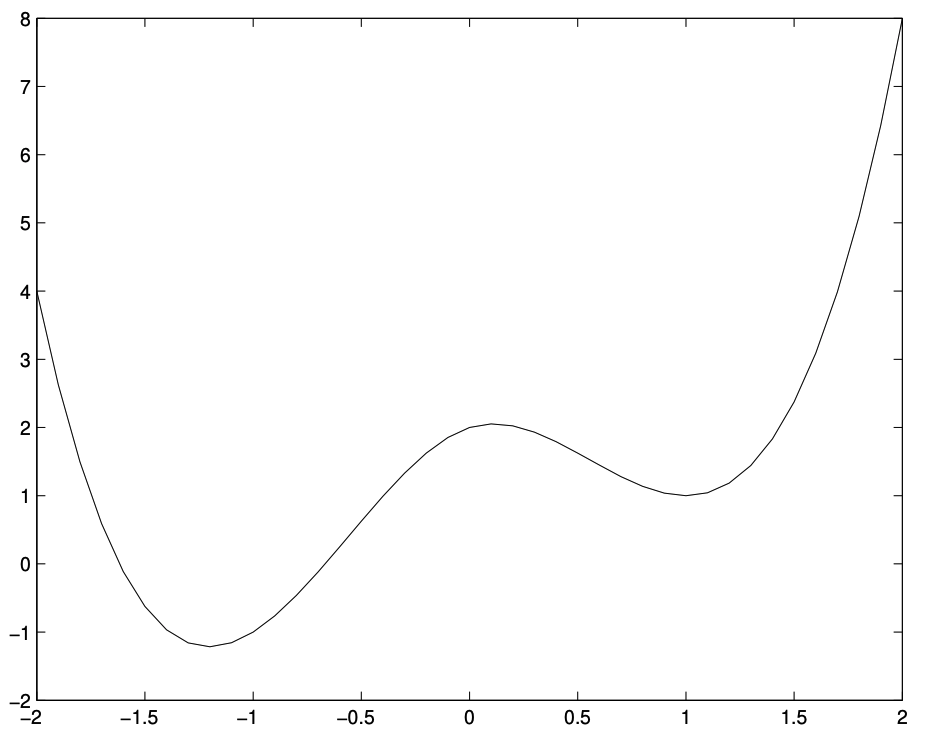
\includegraphics[width=0.45\textwidth]{Figures/spline.png}
    \caption{Spline interpolation}
\end{figure}

\begin{minted}[frame=single,framerule=1pt,  rulecolor=\color{gray}]{matlab}
>> [sp] = spline(x,y)
sp = 
      form: 'pp'
    breaks: [-2 -1 0 1 2]
     coefs: [4x4 double]
    pieces: 4
     order: 4
       dim: 1
\end{minted}

\begin{itemize}
    \item \texttt{spline}: returns the spline structure
    \item \texttt{interp1}: 1-D interpolation and returns the approximated values at the query points.
\end{itemize}

\section{Approximation}

